\subsection{The Muon Spectrometer}
\label{sec:ms}

Surrounding the calorimeters is the muon spectrometer (MS)~\cite{CERN-LHCC-97-022}, responsible
for the detection of high-momentum, minimum-ionizing muons originating from the $pp$ interaction.
The MS is based on the magnetic deflection of muon tracks, allowing for their
momentum determination.
The bending of the muon trajectories is provided by the large
superconducting air-core toroid magnet system, illustrated in Figure~\ref{fig:atlas_magnet_system},
consisting of a large barrel toroid over the range $\lvert \eta \rvert < 1.4$
and end-cap toroid systems in the range $1.6 < \lvert \eta \rvert < 2.7$.
The superconducting toroid magnet provides an average field of $4\,$T.
The magnetic field bending strength is roughly constant in $\eta$, except in the
region in which the transition between the barrel and end-cap toroids takes place
($1.4 < \lvert \eta \rvert < 1.6$).
A view of the ATLAS detector is shown in Figure~\ref{fig:atlas_in_cavern},
where it can be seen that the volume enclosed by the MS takes up most of the available volume
outside of the calorimeter systems in the underground experimental cavern at Point 1.
It should be noted that the overall design of the superconducting toroid structure,
dictated by the performance requirements of the MS, is what gives ATLAS its large size and essentially
drove the original design of all subdetectors discussed in the previous sections.


\begin{figure}[!htb]
    \begin{center}
        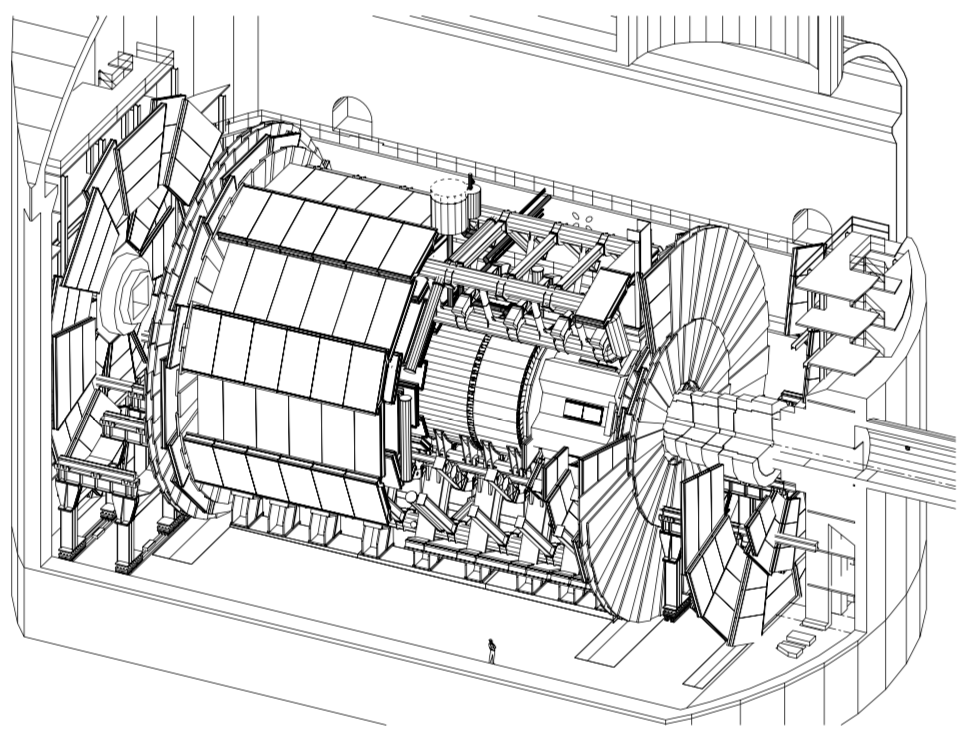
\includegraphics[width=0.8\textwidth]{figures/chapter2/atlas_in_cavern}
        \caption{
            A view of the ATLAS detector inside the underground experimental area
            UX15.
            The cut-away view exposes the toroid structure and
            calorimeter system.
            Notice that the outermost muon stations in the forward regions are located
            at the extreme ends of the cavern.
        }
        \label{fig:atlas_in_cavern}
    \end{center}
\end{figure}
\FloatBarrier

There are four types of gaseous radiation detector used in the MS, and their chamber
layout is based on the concept of projective towers.
The chambers follow the structure of the toroid magnet structure and have a 16-fold segmentation
in azimuth, shown in Figure~\ref{fig:muon_segmentation}.
They are arranged in large and small sectors, with the large sectors covering
the regions between the coils of the toroid and the small sectors the azimuthal range
in which the coils sit.
The detector types can be broken into two classes and are either
\textit{precision} or \textit{trigger} chambers.
The precision chambers are composed of Monitored Drift Tube (MDT)~\cite{Bauer:2016gyg} and Cathode Strip Chamber (CSC)~\cite{Argyropoulos:2009zz}
detectors and allow for
the precise measurement the muon tracks as they traverse the MS, specifically the
precise measurement in the bending plane of these tracks so as to allow for accurate
determination of the muon momenta through their curvature.
The trigger chambers are composed of Resistive Plate Chamber (RPC)~\cite{Aielli:2006hg} and Thin Gap Chamber (TGC)~\cite{Majewski:1984ag}
detectors and have fast signal formation and readout times, allowing for
accurate assignment of a passing muon to a specific $pp$ bunch crossing.
Both types of detectors exist in the barrel and end-cap sections of the
MS and there are typically at least three layers of precision-type chambers over the
entire $\lvert \eta \rvert$ range of the MS in order to allow for the sagitta measurement
of the muon tracks necessary for momentum determination.
The number of precision chamber  hits over the entire range in $\eta-\phi$ of the MS
is shown on the left side of Figure~\ref{fig:muon_nchambers_crossed}. 
In the regions $\lvert \eta \rvert \sim 0$ and $\lvert \eta \rvert \sim 1.2$ there
are noticeable drops in chamber coverage in order to allow for ID and calorimeter
services and in the transition region between the barrel and end-cap, respectively,
as seen on the right side of Figure~\ref{fig:muon_nchambers_crossed}.


\begin{figure}[!htb]
    \begin{center}
        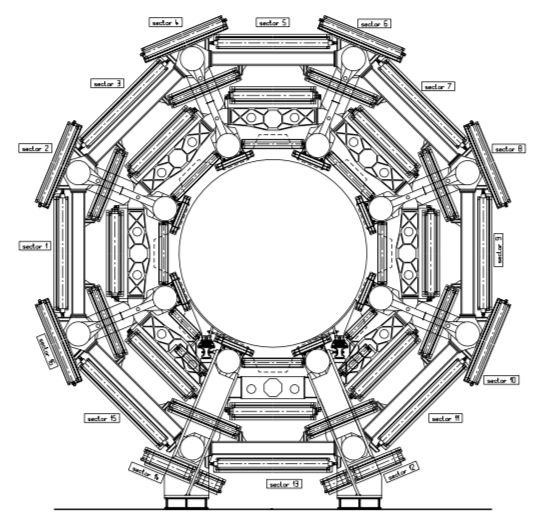
\includegraphics[width=0.4\textwidth]{figures/chapter2/muon_spec/atlas_muon_barrel}
        \raisebox{0.4cm}{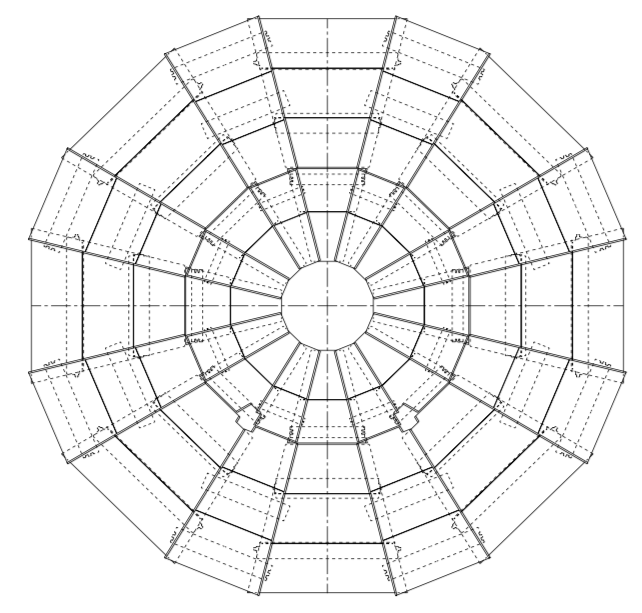
\includegraphics[width=0.35\textwidth]{figures/chapter2/muon_spec/atlas_muon_endcap}}
        \caption{
            View of the 16-fold segmentation of the muon spectrometer in the barrel (\textit{left})
            and end-cap (\textit{right}).
            Clearly seen in both is the arrangment of the detector chambers into large and
            small sectors, allowing for complete coverage in azimuth.
            The view of the end-cap is that only of the MDT chambers located at $z\approx13$\,m.
        }
        \label{fig:muon_segmentation}
    \end{center}
\end{figure}

\begin{figure}[!htb]
    \begin{center}
        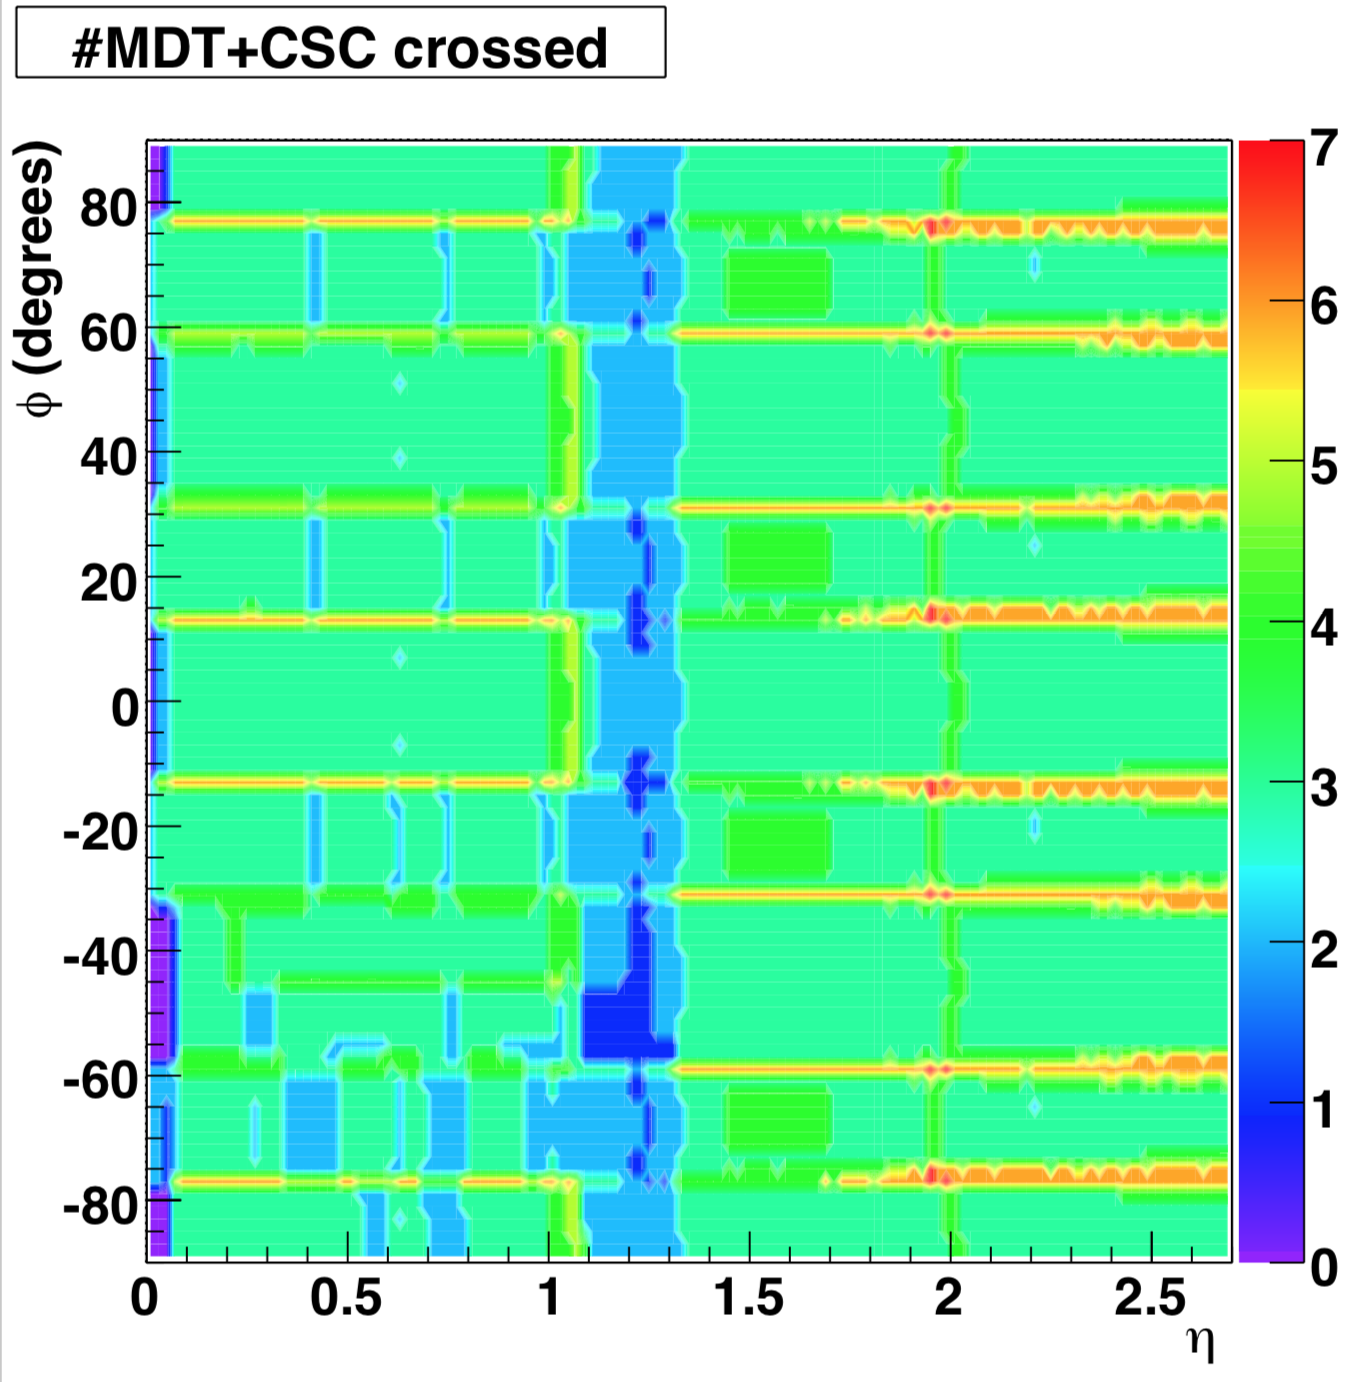
\includegraphics[width=0.4\textwidth]{figures/chapter2/muon_spec/atlas_ms_nchamber_crossed}
        \raisebox{0.6cm}{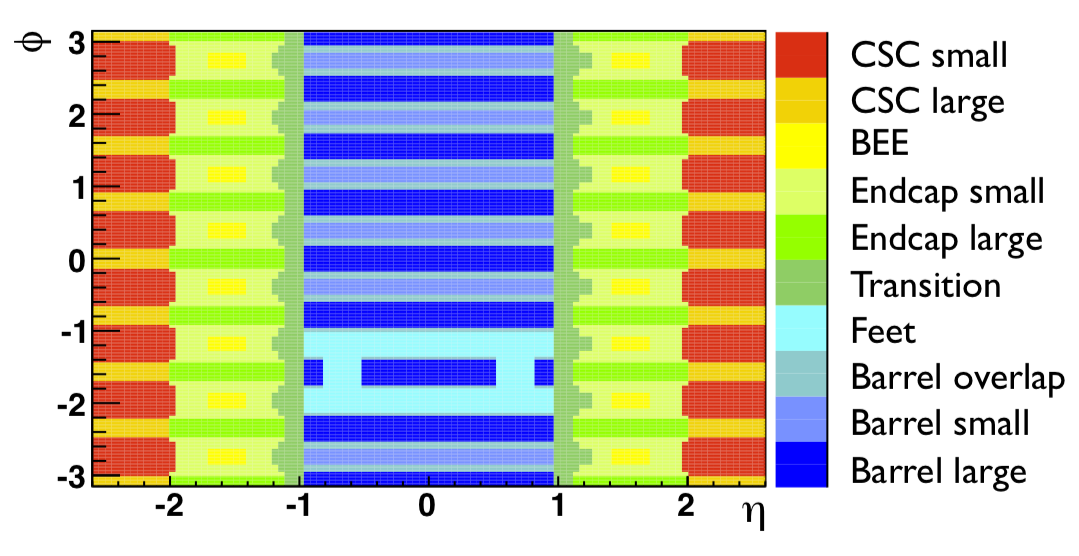
\includegraphics[width=0.58\textwidth]{figures/chapter2/muon_spec/atlas_muon_overlap}}
        \caption{
            \textit{Left}: Number of precision muon chambers (MDT and CSC) traversed by a muon passing through the muon
                spectrometer as a function of $\eta$ and $\phi$.
                The regions of high numbers of crossings ($>4$) correspond to the regions of overlap
                between the large and small sectors.
            \textit{Right}: Location in $\eta-\phi$ of several regions of the MS.
        }
        \label{fig:muon_nchambers_crossed}
    \end{center}
\end{figure}
\FloatBarrier

The layout of the muon chambers and the corresponding detector technologies
in the barrel and end-cap sections is shown in Figure~\ref{fig:muon_plan_view_eta}.
Here we will briefly describe each, starting with those in the barrel section.

\begin{figure}[!htb]
    \begin{center}
        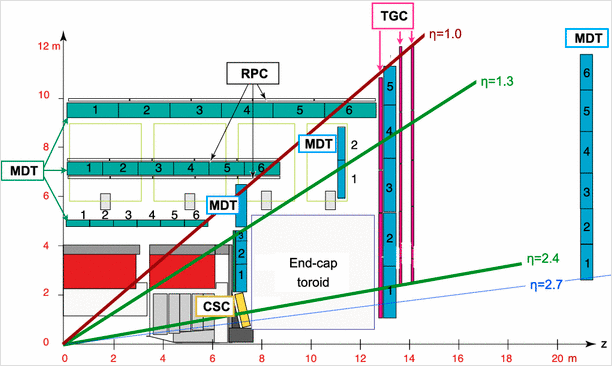
\includegraphics[width=0.8\textwidth]{figures/chapter2/muon_spec/atlas_muon_plan_view_eta}
        \caption{
            A view in the $r-z$ plane of a quadrant of the muon spectrometer (MS).
            Indicated by color are the four detector technologies used in the MS:
            MDT (blue), RPC (grey), TGC (red), and CSC (yellow).
            The light grey boxes at $6 < r < 9$\,m indicate the location of the
            barrel toroid structures.
            Also shown are the envelopes in $\lvert \eta \rvert$ of the barrel,
            small wheel, and big wheel sections of the MS.
        }
        \label{fig:muon_plan_view_eta}
    \end{center}
\end{figure}
\FloatBarrier

\subsubsection{Muon Spectromter: Barrel}
\label{sec:ms_barrel}

The muon chambers in the barrel section of the MS are rectangular in shape and arranged in 3 cylindrical shells,
concentric about and parallel to the beam-axis at radial distances of 5, 7.5, and 10.5\,m (see Figure~\ref{fig:muon_segmentation}).
The precision chambers in the barrel section are composed of MDT chambers
with tubes perpendicular to the beam-axis and parallel to the toroidal magnetic field,
allowing for precision measurement along $\eta$.
The MDT tubes are $3\,$cm in diameter and contain a 93\% Ar -- 7\% CO$_2$ gas mixture
with a single tungsten-rhenium wire operated at $3$\,kV.
Traversal of a minimium ionising particle (MIP) ionises the gas within the tube,
and the signal of the resulting ionisation charge is read out.
The typical spatial resolution of a single MDT tube is below $100\,\micron$.
The MDT chambers are built as multi-layers of many MDT tubes which allows for the improvement
of the spatial resolution down to $50\,\micron$ when the information from the individual layers is combined.
An MDT double multi-layer chamber is shown in Figure~\ref{fig:mdt_chamber}.
Also illustrated in this figure is the principle by which the tube hits in a given MDT
multi-layer are used to form tracklets which aid in the process of muon track-building.

\begin{figure}[!htb]
    \begin{center}
        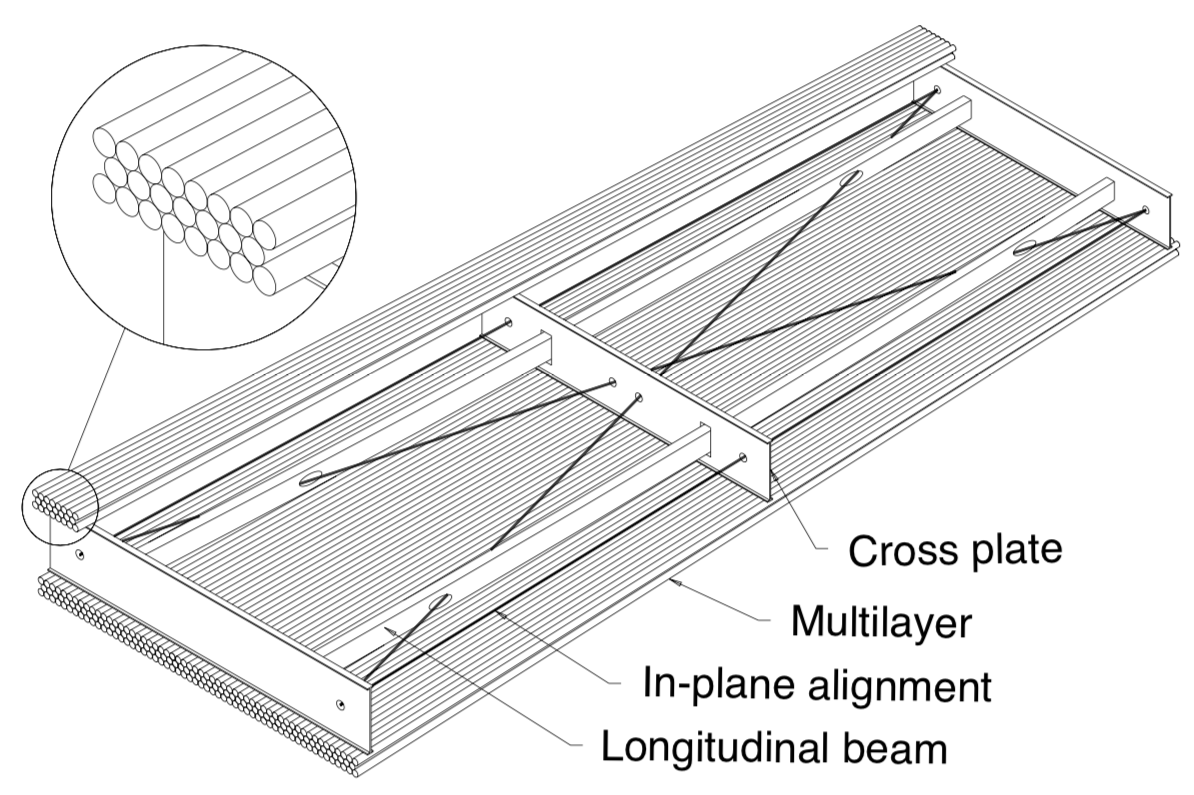
\includegraphics[width=0.5\textwidth]{figures/chapter2/muon_spec/mdt_chamber}
        \raisebox{1.22cm}{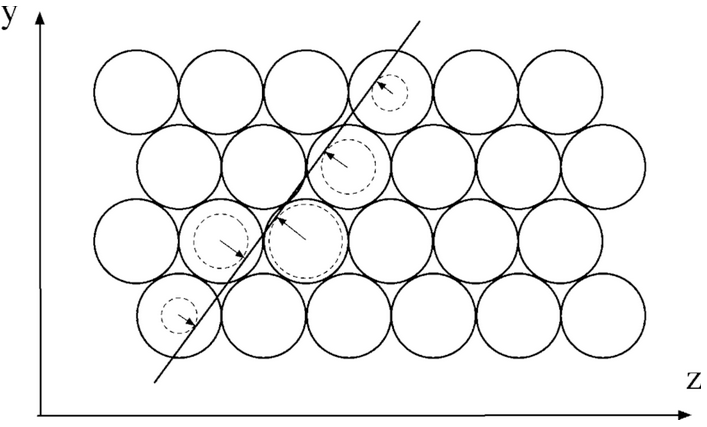
\includegraphics[width=0.32\textwidth]{figures/chapter2/muon_spec/mdt_trackfit}}
        \caption{
            \textit{Left}: Illustration of a double-multilayer MDT chamber with its internal alignment
                and support structure exposed. A zoom-in on the multilayer of MDT tubes is shown.
            \textit{Right}: Illustration of the multilayer MDT tracklet-fitting algorithm~\cite{MDTtrackfit}.
        }
        \label{fig:mdt_chamber}
    \end{center}
\end{figure}

The chambers responsible for constructing muon trigger primitives in the MS barrel
are the RPC chambers, whose principle of operation is shown on the left of Figure~\ref{fig:muon_trigger_chamber}. 
The RPC gap is 2\,mm, filled with tetrafluorethane (C$_2$H$_2$F$_4$), and is lined with
parallel plate electrodes operated at a potential difference of 9.8\,kV. This high operating
potential and gas mixture allows for a timing resolution of 2\,ns. Readout strips in $x$ and $y$
collect the induced charge from the ionisation events within the gap and provide
additional spatial information for track and trigger-primitive building.

\subsubsection{Muon Spectrometer: End-cap}
\label{sec:ms_endcap}

The end-cap muon chambers, located in $1 < \lvert \eta \rvert < 2.7$, are arranged
in 4 rings --- \textit{wheels} ---  extending radially and concentric with the beam axis at $z \approx 7.5, 10, 14, 22$\,m
from the $pp$ interaction point.
The wheel at $z\approx 7.5$\,m, located on the IP-side of the end-cap toroid, is referred to as the `Small Wheel' and those at $z>10$\,m are
referred to as the `Big Wheels'.
That at $z\approx 10$\,m, situated above the end-cap toroid, is an intermediate muon station composed of MDT chambers and has generally lower coverage than the
Small and Big Wheels.

As in the barrel section, the primary precision measurement in the end-caps is provided
by MDT chambers which are located in all four wheels of the end-cap.
The MDT tubes are oriented azimuthally in order to obtain precision measurement in $\eta$.
At the region $2 < \lvert \eta \rvert < 2.7$, in the innermost muon station
in the end-cap that experiences the highest background rates,
the precision muon measurement is provided by the CSC chambers at low radii.
The CSC detectors are multi-wire proportional chambers, illustrated in Figure~\ref{fig:csc_chamber},
with cathode strips perpendicular to anode wires and operated with Ar/CO$_2$/CF$_4$ gas mixtures.
Passing MIPs result in ionisation events whose signals along the strips and wires are
subsequently readout.
As compared to the MDT chambers, the CSC detectors can resolve spatial information in both $\eta$ and $\phi$
and, due to their relatively high granularity readout structure, can sustain the higher
background rates experienced in this very forward region of the detector.
The CSC sectors are multi-layered (4-layers) and can achieve spatial hit resolutions on the order
of $60\,\micron$.

The trigger chambers in the end-cap are composed of the TGC detectors.
Like the CSC, the TGC is a multi-wire proportional chamber with a gas mixture
of CO$_2$ and $n$-pentante ($n$-C$_5$H$_{12}$).
An illustration of the operating principles of a TGC detector is shown in Figure~\ref{fig:muon_trigger_chamber}.
The graphite cathodes and wires, with $1.4$\,mm separation, are held at a potential
difference of $2.9$\,kV.
This high potential difference and anode/cathode geometry allows for signals to be readout
with a timing resolution of 4\,ns.
The signals from the drift electrons, collected along the wires, and the induced
charge on the strips located behind the G-10 layer are read out and provide
two-dimensional spatial information that can be used both in track and trigger-primitive building.


\begin{figure}[!htb]
    \begin{center}
        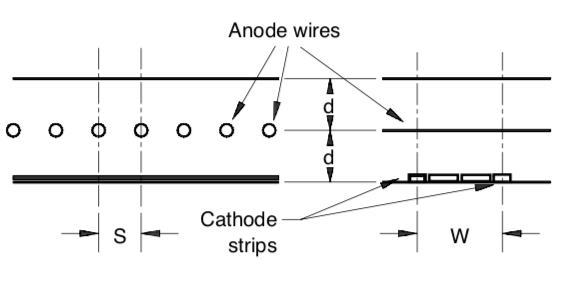
\includegraphics[width=0.55\textwidth]{figures/chapter2/muon_spec/csc_chamber}
        \caption{
            Diagram showing the main components of a cathode-strip chamber (CSC).
            On the \textit{left} (\textit{right}) is a view parallel (perpendicular) to the anode
            wires and perpendicular (parallel) to the cathode strips.
        }
        \label{fig:csc_chamber}
    \end{center}
\end{figure}

%\subsubsection{Muon Trigger Chambers}
%\label{sec:muon_trigger}

\begin{figure}[!htb]
    \begin{center}
        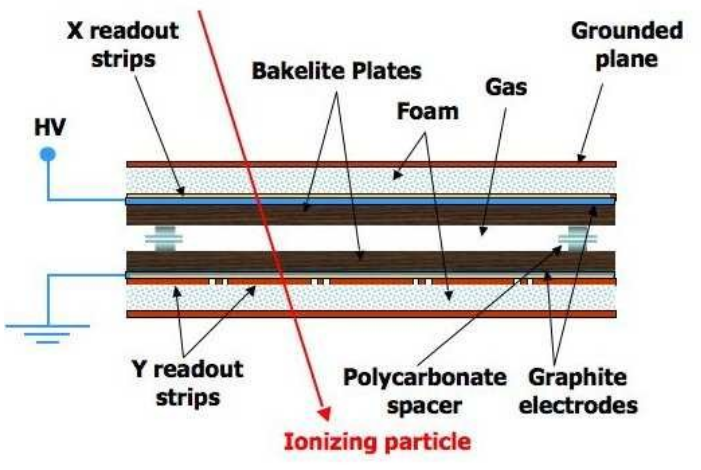
\includegraphics[width=0.5\textwidth]{figures/chapter2/muon_spec/rpc_chamber}
        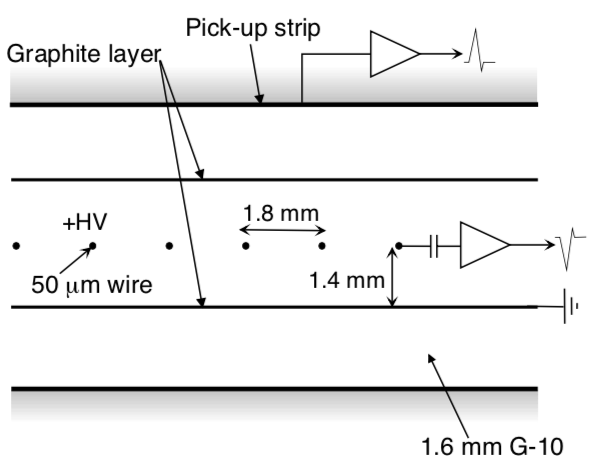
\includegraphics[width=0.38\textwidth]{figures/chapter2/muon_spec/tgc_chamber}
        \caption{
            Muon trigger chambers.
            \textit{Left}: Illustration of a resistive plate chamber (RPC) and its principle of operation.
            \textit{Right}: Diagram showing the main components of a thin-gap chamber (TGC).
        }
        \label{fig:muon_trigger_chamber}
    \end{center}
\end{figure}
